\documentclass[12pt]{article}

% Packages for formatting
\usepackage{amsmath, amssymb}
\usepackage{listings}
\usepackage{xcolor}
\usepackage{graphicx}
\usepackage[margin=1in]{geometry}

% Python code style
\lstdefinestyle{mypython}{
  language=Python,
  basicstyle=\ttfamily\footnotesize,
  keywordstyle=\color{blue},
  commentstyle=\color{gray},
  stringstyle=\color{orange},
  showstringspaces=false,
  breaklines=true,
  frame=single,
  numbers=left,
  numberstyle=\tiny\color{gray},
  tabsize=4
}

\begin{document}

\title{Report on Crude Oil Price Prediction using Black-Scholes Concepts and Brownian Motion}
\author{}
\date{}
\maketitle

\section{Model Explanation: Black-Scholes Concepts and Brownian Motion}

\subsection{Brownian Motion}
Brownian motion is a mathematical model used to describe the random movement of particles suspended in a fluid.  
In finance, it is adapted to model the random fluctuations of asset prices over time. The key idea is that price movements are unpredictable in the short term and can be represented as a random walk.  

A common model for asset prices is \textbf{Geometric Brownian Motion (GBM)}, where the logarithm of the asset price follows a random walk with a drift. The stochastic process underlying the Black-Scholes model is:

\[
dS = \mu S \, dt + \sigma S \, dW_t
\]

Where:  
- \( S \): Asset price  
- \( \mu \): Drift (expected rate of return)  
- \( \sigma \): Volatility (standard deviation of returns)  
- \( dt \): Small time interval  
- \( dW_t \): Wiener process, representing random shock  

\subsection{Black-Scholes Model Concepts}
The Black-Scholes model is a famous mathematical model for pricing European-style options.  
Its underlying assumption is that asset prices follow a random walk with constant drift and volatility.  

In this task, we borrow the idea from Black-Scholes that volatility (\( \sigma \)) is a key parameter in determining the magnitude of random price movements. Historical data is used to estimate volatility, which is then applied to simulate future price movement using Brownian motion.  

---

\section{Explanation of Code Steps}

The Python code predicts crude oil spot price one day ahead by following these steps:

\subsection{1. Data Loading and Preparation}
\begin{itemize}
  \item Load historical crude oil price data into a pandas DataFrame.
  \item Convert the \texttt{observation\_date} column to datetime and set as index.
  \item Ensure the \texttt{DCOILWTICO} column is numeric.
  \item Filter data to last 10 years.
\end{itemize}

\subsection{2. Volatility Calculation}
\begin{itemize}
  \item Calculate daily returns using \texttt{pct\_change()}.
  \item Compute daily volatility (std. dev. of returns).
  \item Annualize volatility:  
  \[
  \sigma_{annual} = \sigma_{daily} \times \sqrt{252}
  \]
\end{itemize}

\subsection{3. Price Prediction (One Day Ahead)}
\begin{itemize}
  \item Retrieve the last available price.
  \item Define time step: \( dt = \tfrac{1}{252} \).
  \item Generate a random shock \( Z \sim N(0,1) \).
  \item Predict price using Geometric Brownian Motion:
  \[
  S_{t+dt} = S_t \times \exp\Big( (\mu - 0.5\sigma^2)dt + \sigma\sqrt{dt}Z \Big)
  \]
  \item Here, \(\mu = 0\) for simplicity in a one-day forecast.
\end{itemize}

---

\section{Python Code}

\begin{lstlisting}[style=mypython]
import pandas as pd
import numpy as np
from datetime import datetime, timedelta

# Load the data from the CSV file
df_oil_prices = pd.read_csv("/content/wti crude oil price.csv")

# Convert to numeric and clean data
df_oil_prices['DCOILWTICO'] = pd.to_numeric(df_oil_prices['DCOILWTICO'], errors='coerce')
df_oil_prices.dropna(subset=['DCOILWTICO'], inplace=True)

# Ensure datetime index
df_oil_prices['observation_date'] = pd.to_datetime(df_oil_prices['observation_date'])
df_oil_prices.set_index('observation_date', inplace=True)

# Filter for last 10 years
current_date = datetime.now()
start_date_10_years_ago = current_date - timedelta(days=10*365)
df_recent_prices = df_oil_prices[df_oil_prices.index >= start_date_10_years_ago].copy()

# Calculate returns and volatility
df_recent_prices['Daily_Return'] = df_recent_prices['DCOILWTICO'].pct_change()
daily_volatility = df_recent_prices['Daily_Return'].std()
annualized_volatility = daily_volatility * np.sqrt(252)

# Last price
last_price = df_recent_prices['DCOILWTICO'].iloc[-1]

# Time step
time_step_days = 1
time_step_years = time_step_days / 252.0

# Brownian motion simulation
drift = 0
np.random.seed(42)
z = np.random.normal(0, 1)

# Predicted price
predicted_price = last_price * np.exp(
    (drift - 0.5 * annualized_volatility**2) * time_step_years
    + annualized_volatility * np.sqrt(time_step_years) * z
)
\end{lstlisting}

---

\section{Historical and Predicted Prices Chart}

\begin{figure}[ht!]
    \centering
    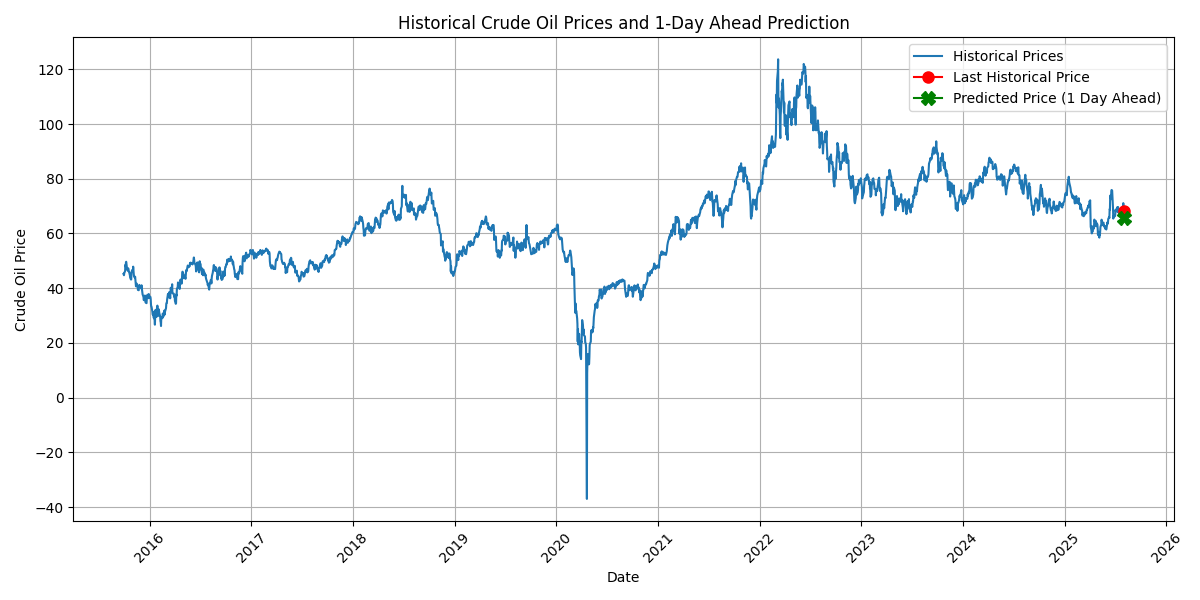
\includegraphics[width=\textwidth]{crude_oil_price_prediction_chart.png}
    \caption{Historical Crude Oil Prices and 1-Day Ahead Prediction}
\end{figure}

\end{document}
